\chapter{Experimental Setup and Results}
\label{ch:experimental-results}

%TODO Add a section illustrating the implementation; giving some examples of how clustering algorithms are used to define a state-space and learn an MDP based on likelihood maximization and how this MDP is used to navigate the robot in an environment.

%\begin{itemize}
%	\item Introduction about application and high-level explanation of what we'll be looking into
%\end{itemize}

In \autoref{ch:methodology} a framework was proposed for finding an optimal \acrshort{acr:mdp} for planning problems that involve uncertainty given a dataset describing the dynamics of the system under consideration.
The framework aims to achieve this by posing the adjustment of the parameters of model learning algorithms as an optimization task in which the yielded performance is to be maximized.
The domain of mobile robot navigation, where the problem statement is to navigate a robot between locations as fast as possible, was identified as a potentially suitable application.
This chapter discusses the experiments that were conducted to evaluate the framework for this application and the results that were obtained accordingly.
First of all, \autoref{sec:setup} elaborates upon the setup for the experiments, discussing the relevant details on the implementation of the framework for this application and the software and other resources used.
Subsequently, \autoref{sec:scenarios} discusses the different configurations that shall be used to test the framework.
This for instance involves various combinations of learning algorithms and different settings of the weight factor $\beta$ on different environments.
In, \autoref{sec:results} the results obtained for these different configurations are presented, inspected and compared to one another, after which the most notable conclusions that can be drawn are discussed.

\section{Setup}
\label{sec:setup}

For our experiments we made an implementation of the framework in the form of a module that can be used to learn an optimal \acrshort{acr:mdp} for the navigation of a mobile robot.
This implementation allows the control of a mobile robot in simulations by an \acrshort{acr:mdp} and a corresponding policy.
The model values assessed from these simulations are used to find a globally maximizing parameter-settings of the learning algorithm used.
In this section we will describe the implementation in detail and how it is used in our experiments to find performance-maximizing \acrshortpl{acr:mdp} for a mobile robot in an office environment.

\subsection{Software}
\label{sec:software}

In this section we discuss the software that is used in the implementation of our optimization module. 
An overview of the main packages used for this implementation is presented in \autoref{tab:software-packages}.
In the remainder of this section, we briefly explain for what part of the implementation each of these packages are used, and support the choices made where necessary.

\begin{table}[pt]
\caption{Software packages used for the implementation of the model learning framework for mobile robot navigation.}
\label{tab:software-packages}\centering
\begin{tabular}{|l|l|l|}
	\hline%
	\textbf{Package Name} & \textbf{Version} & \textbf{Purpose} \\
	\hline
	\texttt{bayesian-optimization} & 0.4.0 & Bayesian optimization \\
	\texttt{matplotlib} & 1.3.1 & Plotting and visualizing robot actions \\
	\texttt{numpy} & 1.12.1 & Array data storage and manipulation\\ 
	\texttt{pymdptoolbox} & 4.0\_b3 & \acrshort{acr:mdp} planning algorithms \\
	\texttt{ros-indigo-strands-desktop} & 0.0.14 & Simulation software and environments\\
	\texttt{scikit-learn} & 0.18.1 & Machine learning algorithms \\ \hline
\end{tabular}
\end{table}

\subsubsection{Python Libraries}
\label{sec:software-packages}
The module has been implemented in Python 2.7, due to its easily usable libraries for machine learning and plotting and other widely available packages, but also because of its convenient capability of interacting with the simulation software used.

For \acrshort{acr:mdp} planning, the \texttt{pymdptoolbox} library \cite{cordwellpymdptoolbox}, is used, which implements various planning algorithms for discrete-time \acrshortpl{acr:mdp}. 
To solve for optimal policies in learned \acrshortpl{acr:mdp} we rely on this library and apply the \acrshort{acr:vi} algorithm with a discount factor of $\gamma = 0.95$.
%Given the matrices with the transition probabilities and rewards and algorithm-parameters like a discount factor $\gamma$, these planning algorithms can produce a policy vector and a corresponding value function.

For the machine learning algorithms used, we employ the \texttt{scikit-learn} library. These algorithms include $k$-Means clustering and \acrfull{acr:gmm}.

For \acrlong{acr:bo} the \texttt{bayesian-optimization} library \cite{nogueirabayesianoptimization} has been employed. This library offers an implementation of the \acrshort{acr:bo} procedure based on a \acrshort{acr:gp} prior including the implementation of the most-used acquisition functions such as \acrshort{acr:mpi}, \acrshort{acr:mei} and \acrshort{acr:gp-ucb}.

The further main Python packages used, have been listed in \autoref{tab:software-packages} and include \texttt{numpy} for the storage and manipulation of arrays and matrices used in the implementation and \texttt{matplotlib} for creating the various plots shown in this chapter.

\subsubsection{Simulator and Mobile Robot}
\label{sec:simulator}

%TODO Maybe remove these figures and rather show a figure of the simulator with the SCITOS robot?
% Make figure with two subfigures
\begin{figure}[t]
\centering
\begin{minipage}{0.4\textwidth}
	\centering
	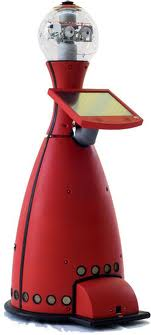
\includegraphics[width=0.3\linewidth]{scitosa5_1_model}
	\captionof{figure}{The SCITOS-A5, mobile service robot by Metralabs GmbH \cite{Metralabs}}
	\label{fig:scitosa5}
\end{minipage}
\qquad
\begin{minipage}{0.4\textwidth}
	\centering
	\vspace{23pt}
	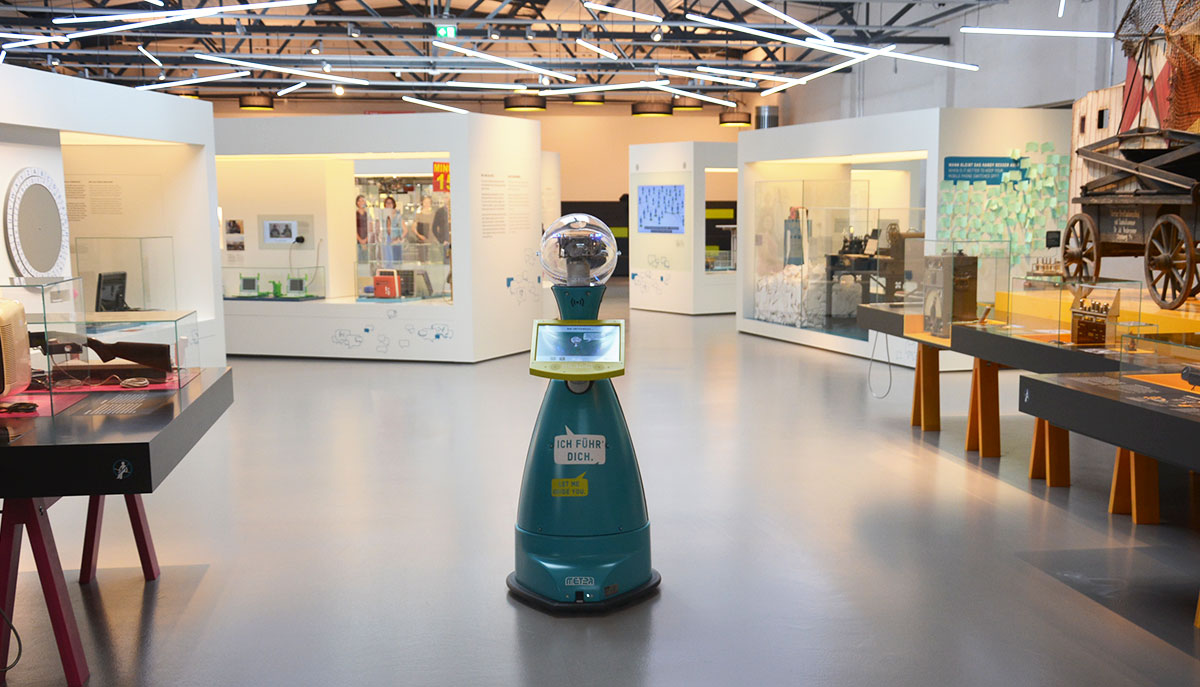
\includegraphics[width=1.1\linewidth]{scitosa5_2_TIM}
	\vspace{-10pt}
	\captionof{figure}{The SCITOS-A5 in one of its application environments. Shown here is robot \textit{TIM}, used for leading visitors of the German Technical Museum in Berlin through the exhibits \cite{Metralabs}.}
	\label{fig:scitosa5_2}
\end{minipage}
\end{figure}

For performing simulations the \textit{MORSE} simulator \cite{morse_simpar_2012}, a generic simulator for academic robots, has been used in combination with the \textit{ROS} middleware to control the robot in the environment.
The simulations are performed with the Metralabs GmbH \textit{SCITOS-A5} \cite{Metralabs}, depicted in \autoref{fig:scitosa5}, an industry-standard mobile service robot designed specifically for interacting with humans and guiding them to products or exhibits (e.g., see \autoref{fig:scitosa5_2}).
This robot is equipped with several sensors which can be used for navigation and \acrfull{acr:hri}, such as an omni-directional camera, 24 ultrasonic sensors, a collision sensor and a SICK laser range finder \cite{gross2008shopbot}.
As described in \autoref{sec:datasets} we are particularly interested in the odometric capabilities of the robot for the implementation that has been used in our experiments.
The \texttt{strands-desktop} meta-package (developed as part of the \textit{STRANDS} project \cite{hawes2016strands}) was used to obtain all required simulation software mentioned above with ease, in which the environments used in the simulations of our experiments are contained as well.



%
%\vspace{12pt}
%\noindent\fbox{\textbf{TODO:} Not completely finished yet.}

%Software used for the implementation:
%\begin{itemize}
%	\item Programming Language: \textit{Python (2.7)} together with \texttt{scikit-learn}, \texttt{pymdptoolbox}, \texttt{bayesian-optimization} packages + explain what each of them are used for
%	\item Simulator: \textit{Morse}
%	\item Scitos-A5 robot, mobile service robot (plus \textit{short} discussion of what this robot has been used for in the real world)
%	\item Control movements of robot in simulator through \textit{ROS}
%\end{itemize}

\subsection{Dataset Acquisition}
\label{sec:datasets}

\begin{table}[pt]
	\caption{An excerpt of one of the execution traces datasets showing the format of the entries. Each entry stores the pose (\texttt{x}, \texttt{y} and \texttt{yaw}) of the robot based on odometry readings, and the action executed from this pose.}
	\label{tab:datasets-excerpt}\centering
	{\ttfamily
	\begin{tabular}{r|r|r|r}
		x & y & action\_id & yaw \\
		\hline
		2.243550300598145 & 3.1634166240692 & 1 & 0.7840424207077832 \\
		2.890618801116943 & 3.8128550052643 & 7 & -0.8159573629295891 \\
		3.541900634765625 & 3.1447956562042 & 6 & -1.6159579833378268 \\
		3.544688224792481 & 2.1472022533417 & 0 & -0.0326251734671011 \\
%		4.264401435852051 & 2.0662682056427 & 6 & -1.6326265827467716 \\
		... & ... & ... & ...
	\end{tabular}
	}
\end{table}

\begin{table}[pt]
	\caption{Details about the Morse simulation environments used and the size of the gathered datasets consisting of execution traces of the SCITOS-A5 robot.}
	\label{tab:datasets-environments}\centering
	\begin{tabular}{|l|r|r|}
		\hline
		\textbf{Environment Name} & \textbf{Estimated Area (\si{\metre\squared})} & \textbf{Number of Entries in Dataset} \\
		\hline
		\texttt{tum\_kitchen}& \num{100}              &   \num{4370}                                    \\
		\hline
		\texttt{uol\_bl}& \numrange[range-phrase = --]{800}{1000}               & \num{8616}           						\\ \hline          
	\end{tabular}
\end{table}

In order to be able to learn \acrshortpl{acr:mdp} from data and establish the optimization, we should obtain a dataset that  describes the environment the robot will operate in.
This dataset should describe possible robot poses and to what other poses the execution of the possible actions may lead to, in order to properly describe the dynamics of the system.

For our implementation and the experiments that have been carried out, execution traces have been obtained by letting the robot follow a random action policy during which subsequent poses and actions are logged to a file.
This exploration is performed inside the simulator both for a relatively small environment (i.e., \texttt{tum\_kitchen}, based on a university kitchen of the Technical University of M\"unchen) and  large environment (i.e., \texttt{uol\_bl}) obtained from a repository of the \textit{STRANDS} project.

In the exploration a new entry is recorded in a file after each time step of $T = \SI{1.0}{\second}$, which each contain the robot's pose based on odometric readings with its location as $x$ and $y$ position and its orientation described by the $yaw$.
Apart from that each entry also stores the action that is executed next from the current pose.
Thus, accordingly the next entry tells us the robot's pose after the action in the previous entry has been executed.

In \autoref{tab:datasets-excerpt} an excerpt of one of the datasets is shown, which might give a clearer picture of the data that has been gathered and the format in which it has been stored.
The possible actions of the robot correspond to a discrete set of robot movements in $8$ different directions, being \textit{south}, \textit{south-east}, \textit{east}, \textit{north-east}, \textit{north}, \textit{north-west}, \textit{west} and \textit{south-west}.
For example, the first two entries describes the transformation of the robot's pose after trying to make a \textit{south-east} movement (N.B., positive difference in $x$ corresponds to moving south, while positive difference in $y$ corresponds to moving east).
\autoref{tab:datasets-environments} presents additional information about the environments and the size of the datasets gathered accordingly.

%Explain how the data-sets are obtained. 
%- For multiple environments - What is obtained. - How the data is obtained.

\subsection{Framework Implementation}
\label{sec:implementation}

To evaluate the framework proposed in \autoref{ch:methodology}, an implementation was made for the domain of mobile robot navigation.
This implementation optimizes for an \acrshort{acr:mdp} that maximizes the yielded performance of following plans derived from it. That is, it aims to find a model that ensures a mobile robot moves from one location in an environment to another as fast as possible.
In this section the relevant details of each part of the implementation are discussed.

\subsubsection{Learning Step}
\label{sec:learning-step-robot}

For learning discrete-state \acrshortpl{acr:mdp} from the acquired execution traces, a likelihood maximization approach is applied based on a state space obtained from clustering algorithms.
That is, the state-space is first obtained by applying a clustering algorithm (i.e., $k$-means, \acrshort{acr:gmm}) with the given $\theta$ as its parameter-setting and geometric positions of the execution traces as its training set.
Then, a transition probability distribution is fitted on the execution traces, such that an \acrshort{acr:mdp} may be obtained that comprehends the transitions that are possible when actions are performed from any of its states.

As described in \autoref{sec:learning-step} our learning step first learns an \acrshort{acr:mdp} based on the provided parameter-settings and then assesses the corresponding performance/model value.
The model value is assessed based on how fast (i.e., expressed by the number of time-steps) the agent would execute the tasks it is expected to perform when it is employed with the learned \acrshort{acr:mdp}.

For our domain we define each task as navigating from a start location to a goal location in the environment, each presented as a pair of coordinates, as fast as possible.
We translate these tasks into something that can be fed to the learned \acrshort{acr:mdp}, first of all, by setting the initial state of the \acrshort{acr:mdp} to the state predicted by the selected clustering algorithm for the start coordinates.
Similarly, a goal state is obtained, and accordingly a reward function for the \acrshort{acr:mdp} is defined by setting a one-time reward for this state.
To avoid small state spaces (in which goal states do not map directly to true goals) yielding high value, a discrepancy factor is computed and used as described in \autoref{sec:performance-measure}.

For each task, a value function and policy is computed for the \acrshort{acr:mdp} using the \acrshort{acr:vi} algorithm.
Based on the computed value functions and simulations following the corresponding policies, the value $V_\mathcal{M}$ of the learned \acrshort{acr:mdp} $\mathcal{M}$ is computed as in \autoref{eq:vm} of \autoref{sec:performance-measure}.
In the simulations, for each task, the robot is first put at the start location defined by the task and then moves in the direction imposed by the computed policy at each discrete time step.
It repeats this until the goal state has been reached.
At that point, however, the ``true'' goal might not have been reached by the robot.
This is a problem, because if we would quit the simulation as soon as the goal state has been reached, then \acrshortpl{acr:mdp} with state spaces that are too simple would yield high value.
To take this into account, as soon as the robot reaches the goal state, it checks if it is inside a designer-specified range of the goal location.
If not, the robot is moved into the direction of the goal location and the same check is performed again.

To avoid the simulations running endlessly on a certain task, time-outs are defined at which the simulation is quit.
First of all, a (relatively short) \textit{goal time-out} is defined for reaching the goal from the goal state, which clearly cannot take too long.
Secondly, a \textit{stuck time-out} is defined, which starts when the robot remains at the same location after performing an action.
Finally, there is a \textit{global time-out}, that defines the maximum time the robot is allowed to spend on performing a task, taking into account any extra time caused by slipping.

The output of each learning step is the value of the learned model $V_\mathcal{M}$ and the time spent on model learning and planning.
The last being used when the \acrshort{acr:mei-ps} acquisition function is employed in the optimization.
Further, additional data is logged in each iteration, which is the total iteration time, simulation time, model learning time, total planning time and the parameter-setting $\theta$ used.

%% IMPLEMENTATION LEARNING STEP
% Learning algorithm
	% Clustering algorithm
	% Maximum likelihood
% Objective: 
	% Learn MDP for given theta
	% Tasks (initial and goal locations)
	% Turned into reward function -> apply solver (VI) -> obtain value function and policy to use
	% Simulation:
		% Steps
		% Time-outs (1) stuck (2) goal state to reach goal (3) task
	% Output: Model value, time
% Logging

\subsubsection{Optimization Step}
\label{sec:optimization-step-robot}

For the implementation of the framework for this domain we make use of the \acrshort{acr:bo} framework for optimization based on a \acrshort{acr:gp} with a Mat\'ern 5/2 kernel.
As initially there is no knowledge about the model value given a parameter-setting $\theta$, first, a number of random settings are selected for which yielded performance is assessed and stored in an evidence set.
In the following iterations new settings for $\theta$ are chosen with maximum utility in the selected acquisition function, which is repeated for a fixed number of iterations.

For the extension of the framework described in \autoref{sec:cost-effective-optimization} the first phase is executed as an individual optimization procedure, where the model values are solely based on computed value functions and no simulations are performed.
The resulting posterior of this first phase is then used to define the prior for the second phase with the aim of finding a global maximizer faster than without this pre-processing.

%% OPTIMIZATION STEP
% Initial points (random points)
% Stopping criterions


%Details on the implementation; how the framework/routine is implemented for this application. Discuss how the following aspects are taken care of in the implementation:
%\begin{itemize}
%	\item Environments
%	\item Exploration / Data Gathering
%	\item Optimization
%	\item Simulations of following policy
%\end{itemize}

\section{Experiment Configurations}
\label{sec:scenarios}

\begin{table}
	\caption{Settings for goal radius, parameter domain $\Theta$, time-outs and discount factor used for each of the environments in the experiments.}
	\label{tab:designer-settings}\centering
	\begin{tabular}{|l|r|r|r|r|r|r|}
		\hline
		\textbf{Environment} & \textbf{Goal Radius} & \textbf{Parameter} & \textbf{Goal T/O} & \textbf{Stuck T/O} & \textbf{Global T/O} & \textbf{Discount}  \\

		& \textbf{(\si\meter)} & \textbf{Domain $\Theta$} & (\si{\second}) & (\si{\second}) & (\si{\second}) & \textbf{Factor $\gamma$}\\
		\hline
		\texttt{tum\_kitchen} & \num{0.5} & $[2, 300]$ & \num{10} & \num{10} & \num{30} & \num{0.95} \\
		\hline
		\texttt{uol\_bl} & \num{1.0} & $[100, 1000]$ & \num{10} & \num{10} & \num{120} & \num{0.95}\\
		\hline
	\end{tabular}
\end{table}

\begin{table}
	\caption{Details on the different configurations used for the experiments on the base (single phase) framework.}
	\label{tab:configurations-base}\centering
	\begin{tabular}{|l|l|r|l|l|r|}
		\hline
		\textbf{ID} & \textbf{Environment} & \textbf{Weight Factor $\beta$} & \textbf{Acquisition Function} & \textbf{Algorithm} & \textbf{Dataset Used} \\
		\hline 
		1 & \texttt{tum\_kitchen} & 0.0 & \acrshort{acr:mei} & $k$-Means & 100\% \\
		\hline
		2 & \texttt{tum\_kitchen} & 0.0 & \acrshort{acr:mei} & $k$-Means & 75\%  \\
		\hline
		3 & \texttt{tum\_kitchen} & 0.0 & \acrshort{acr:mei} & $k$-Means & 50\% \\
		\hline
		4 & \texttt{tum\_kitchen} & 0.0 & \acrshort{acr:gp-ucb} & $k$-Means & 100\% \\
		\hline
		5 & \texttt{tum\_kitchen} & 0.0 & \acrshort{acr:mei-ps} & $k$-Means & 100\% \\
		\hline
		6 & \texttt{tum\_kitchen} & 0.0 & \acrshort{acr:mei} & \acrshort{acr:gmm} & 100\% \\
		\hline
		7 & \texttt{tum\_kitchen} & 0.0 & \acrshort{acr:gp-ucb} & \acrshort{acr:gmm} & 100\% \\
		\hline
		%6 & \texttt{tum\_kitchen} & 0.0 & \acrshort{acr:gp-ucb} & \acrshort{acr:gmm} & 100\% \\
		%\hline
		8 & \texttt{tum\_kitchen} & 0.25 & \acrshort{acr:mei} & $k$-Means & 100\% \\
		\hline
		9 & \texttt{tum\_kitchen} & 0.50 & \acrshort{acr:mei} & $k$-Means & 100\% \\
		\hline
		10 & \texttt{uol\_bl} & 0.0 & \acrshort{acr:mei} & $k$-Means & 100\% \\
		\hline
		%10 & \texttt{uol\_bl} & 0.0 & \acrshort{acr:mei} & $k$-Means & 75\%  \\
		%\hline
		%11 & \texttt{uol\_bl} & 0.0 & \acrshort{acr:mei} & $k$-Means & 50\% \\
		%\hline
		%12 & \texttt{uol\_bl} & 0.0 & \acrshort{acr:mei} & \acrshort{acr:gmm} & 100\% \\
		%\hline
		11 & \texttt{uol\_bl} & 0.0 & \acrshort{acr:gp-ucb} & $k$-Means & 100\% \\
		\hline
		12 & \texttt{uol\_bl} & 0.0 & \acrshort{acr:mei-ps} & $k$-Means & 100\% \\
		\hline
		%14 & \texttt{uol\_bl} & 0.0 & \acrshort{acr:gp-ucb} & \acrshort{acr:gmm} & 100\% \\
		%\hline
		%15 & \texttt{uol\_bl} & 0.25 & \acrshort{acr:mei} & $k$-Means & 100\% \\
		%\hline
		%16 & \texttt{uol\_bl} & 0.50 & \acrshort{acr:mei} & $k$-Means & 100\% \\
		%\hline
	\end{tabular}
\end{table}

\begin{table}
	\caption{Details on the different configurations used for the experiments on the multiphase framework.}
	\label{tab:configurations-multi}\centering
	\begin{tabular}{|l|l|r|l|l|r|}
		\hline
		\textbf{ID} & \textbf{Environment} & \textbf{Weight Factor $\beta$} & \textbf{Acquisition Function} & \textbf{Algorithm} & \textbf{Dataset Used} \\
		\hline 
		13 & \texttt{tum\_kitchen} & 0.0 & \acrshort{acr:mei} & $k$-Means & 100\% \\
		\hline
		14 & \texttt{tum\_kitchen} & 0.25 & \acrshort{acr:mei} & $k$-Means & 100\% \\
		\hline
		15 & \texttt{tum\_kitchen} & 0.50 & \acrshort{acr:mei} & $k$-Means & 100\% \\
		\hline
		16 & \texttt{uol\_bl} & 0.0 & \acrshort{acr:mei} & $k$-Means & 100\% \\
		\hline
		17 & \texttt{uol\_bl} & 0.25 & \acrshort{acr:mei} & $k$-Means & 100\% \\
		\hline
		18 & \texttt{uol\_bl} & 0.50 & \acrshort{acr:mei} & $k$-Means & 100\% \\
		\hline
	\end{tabular}
\end{table}

In this section an overview is provided of the experiments that have been performed with the robot navigation implementation of the framework.
\autoref{tab:designer-settings} shows the auxiliary settings used in the experiments for aspects like time-outs, parameter domain and goal radius for each of the environments.
Experiments are conducted for both the \textit{base} framework and \textit{multiphase} framework with each of the environments.
The configurations for these experiments are shown in \autoref{tab:configurations-base} and \autoref{tab:configurations-multi} respectively.

The configurations were chosen in such with the aim of being able to identify how the results are affected based on changes in the used acquisition function, weight factor, clustering algorithm and the part of the dataset used.
In each of these experiments data is stored that comprise the generated evidence sets, log-files and the \acrshortpl{acr:mdp} that yield the best performance.
In the next section the obtained results for each of these configurations are shown and discussed accordingly.

%Discuss the different configurations that are to be compared
%\begin{itemize}
%	\item Fixed values for $\beta$-parameter vs. gradually decreasing from $1$ to $0$
%	\item Multiple environments: small (\texttt{tum\_kitchen}); large (\texttt{uol\_bl})
%	\item Model-learning algorithms: direct clustering vs. trajectory clustering; $k$-means vs. GMM
%	\item Data-sets of different sizes
%\end{itemize}

%\noindent Configurations for the basic optimization framework (only based on simulations):
%\begin{itemize}
%	\item Fixed value for $\beta$ (i.e., which weighs $V_\mathit{DTP}$): $0$, $0.25$ and $0.5$
%	\item Acquisition functions: \acrshort{acr:gp-ucb}, \acrshort{acr:mei}
%	\item GMM vs. $k$-Means (vs. trajectory clustering if time available)
%	\item All available data, 75\% and 50\%
%	\item Discount factor: $\gamma = 0.95$
%	\item Small environment: \texttt{tum\_kitchen}; and large environment: \texttt{uol\_bl}
%\end{itemize}
%We need to record: number of iterations, total time passed, optimum found ($\theta_\textnormal{max}$ and $V_{\mathcal{M},\textnormal{max}}$)
%
%\vspace{12pt}
%\noindent For the cost-incremental extension we could try to observe what happens when we decrease $\beta$ gradually over time.
%
%\vspace{12pt}
%\noindent Do we want to do something with `variable resolution' as post-processing step in the experiments?
%
%\vspace{12pt}
%\noindent\fbox{\textbf{TODO:} Table to be added describing the configurations/scenarios for the experiments.}

\section{Results and Discussion}
\label{sec:results}

From the experiments that have been performed according to the configurations presented in \autoref{sec:scenarios} results have been obtained that are discussed in this section.
First, we present and review the results obtained for the experiments that follow the base framework in \autoref{sec:base-framework-results}.
Then, in \autoref{sec:multiphase-framework-results} the results for the multiphase-extension of the framework are presented and discussed. Each of the plots presented in these sections show the resulting posterior that follows from the evidence gathered in the \acrshort{acr:bo} in which $\theta$ is the parameter-setting for model learning and $f$ is the (unknown) objective function mapping these to model values.

\subsection{Base Framework}
\label{sec:base-framework-results}

\afterpage{
	% ID = 1
	\begin{figure}[t!]
		\centering
		\includegraphics[width=0.9\textwidth]{plots/tum_base/plot_b_00__alg_kmeans_pct_100_acq_ei}
		\caption{Plot showing posterior after 20 iterations of the optimization routine for the \texttt{tum\_kitchen} environment, $\beta = 0.0$, $k$-Means, $100\%$ of the dataset used, \acrshort{acr:mei} acquisition function used (Experiment 1).}
		\label{fig:exp1}
	\end{figure}
	% ID = 2
	\begin{figure}[t!]
		\centering
		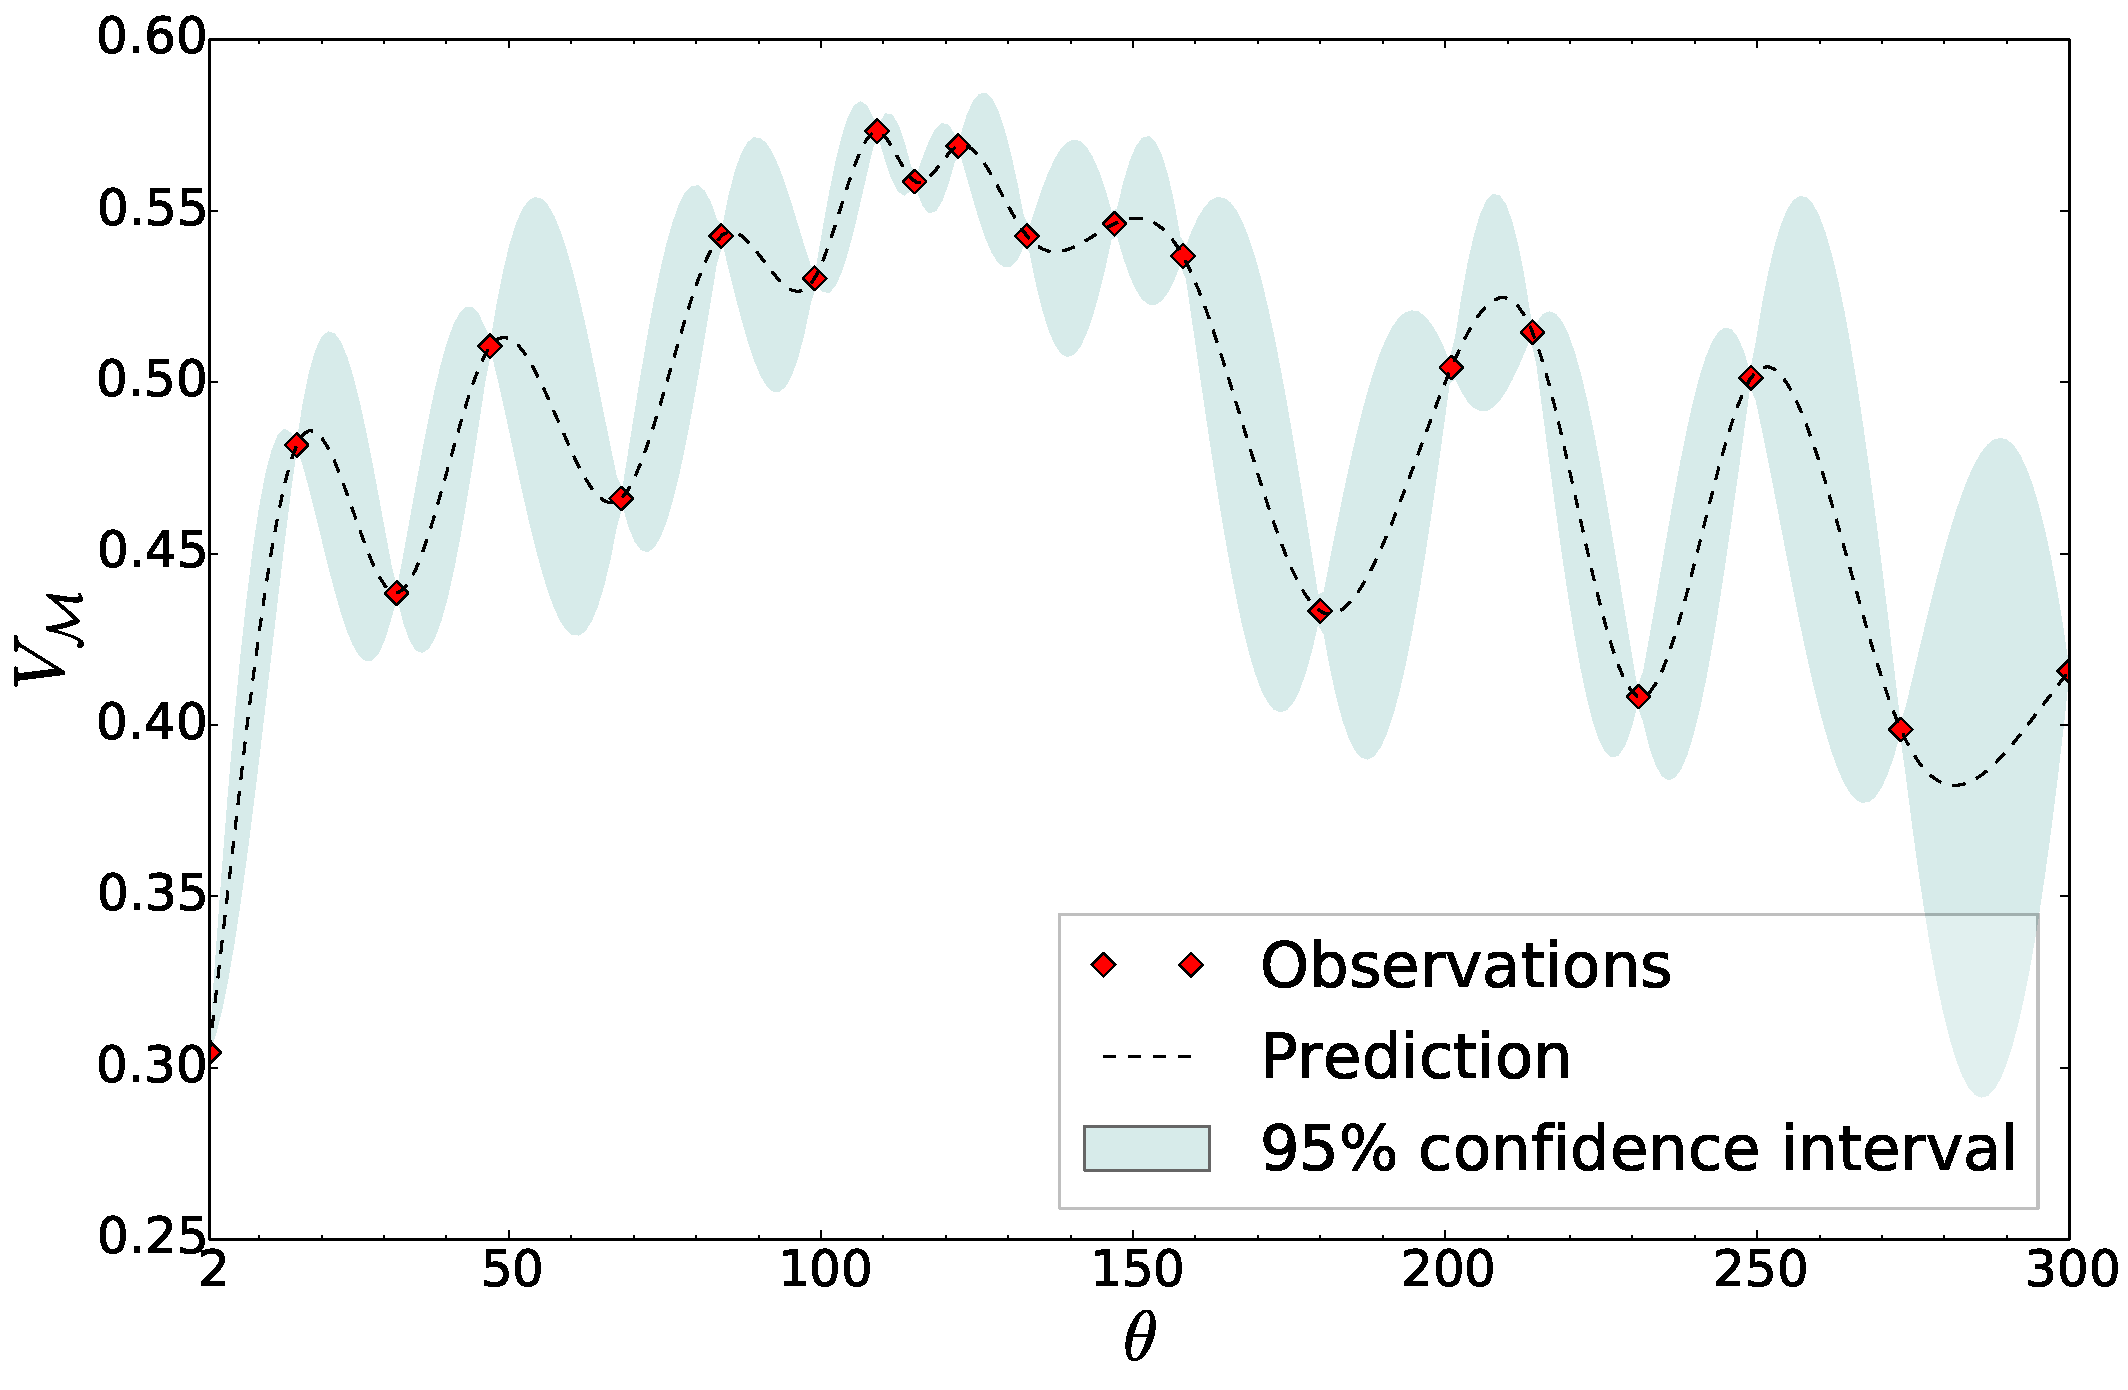
\includegraphics[width=0.9\textwidth]{plots/tum_base/plot_b_00__alg_kmeans_pct_75_acq_ei}
		\caption{Plot showing posterior after 20 iterations of the optimization routine for the \texttt{tum\_kitchen} environment, $\beta = 0.0$, $k$-Means, $75\%$ of the dataset used, \acrshort{acr:mei} acquisition function used (Experiment 2).}
		\label{fig:exp2}
	\end{figure}
	% ID = 3
	\begin{figure}[t!]
		\centering
		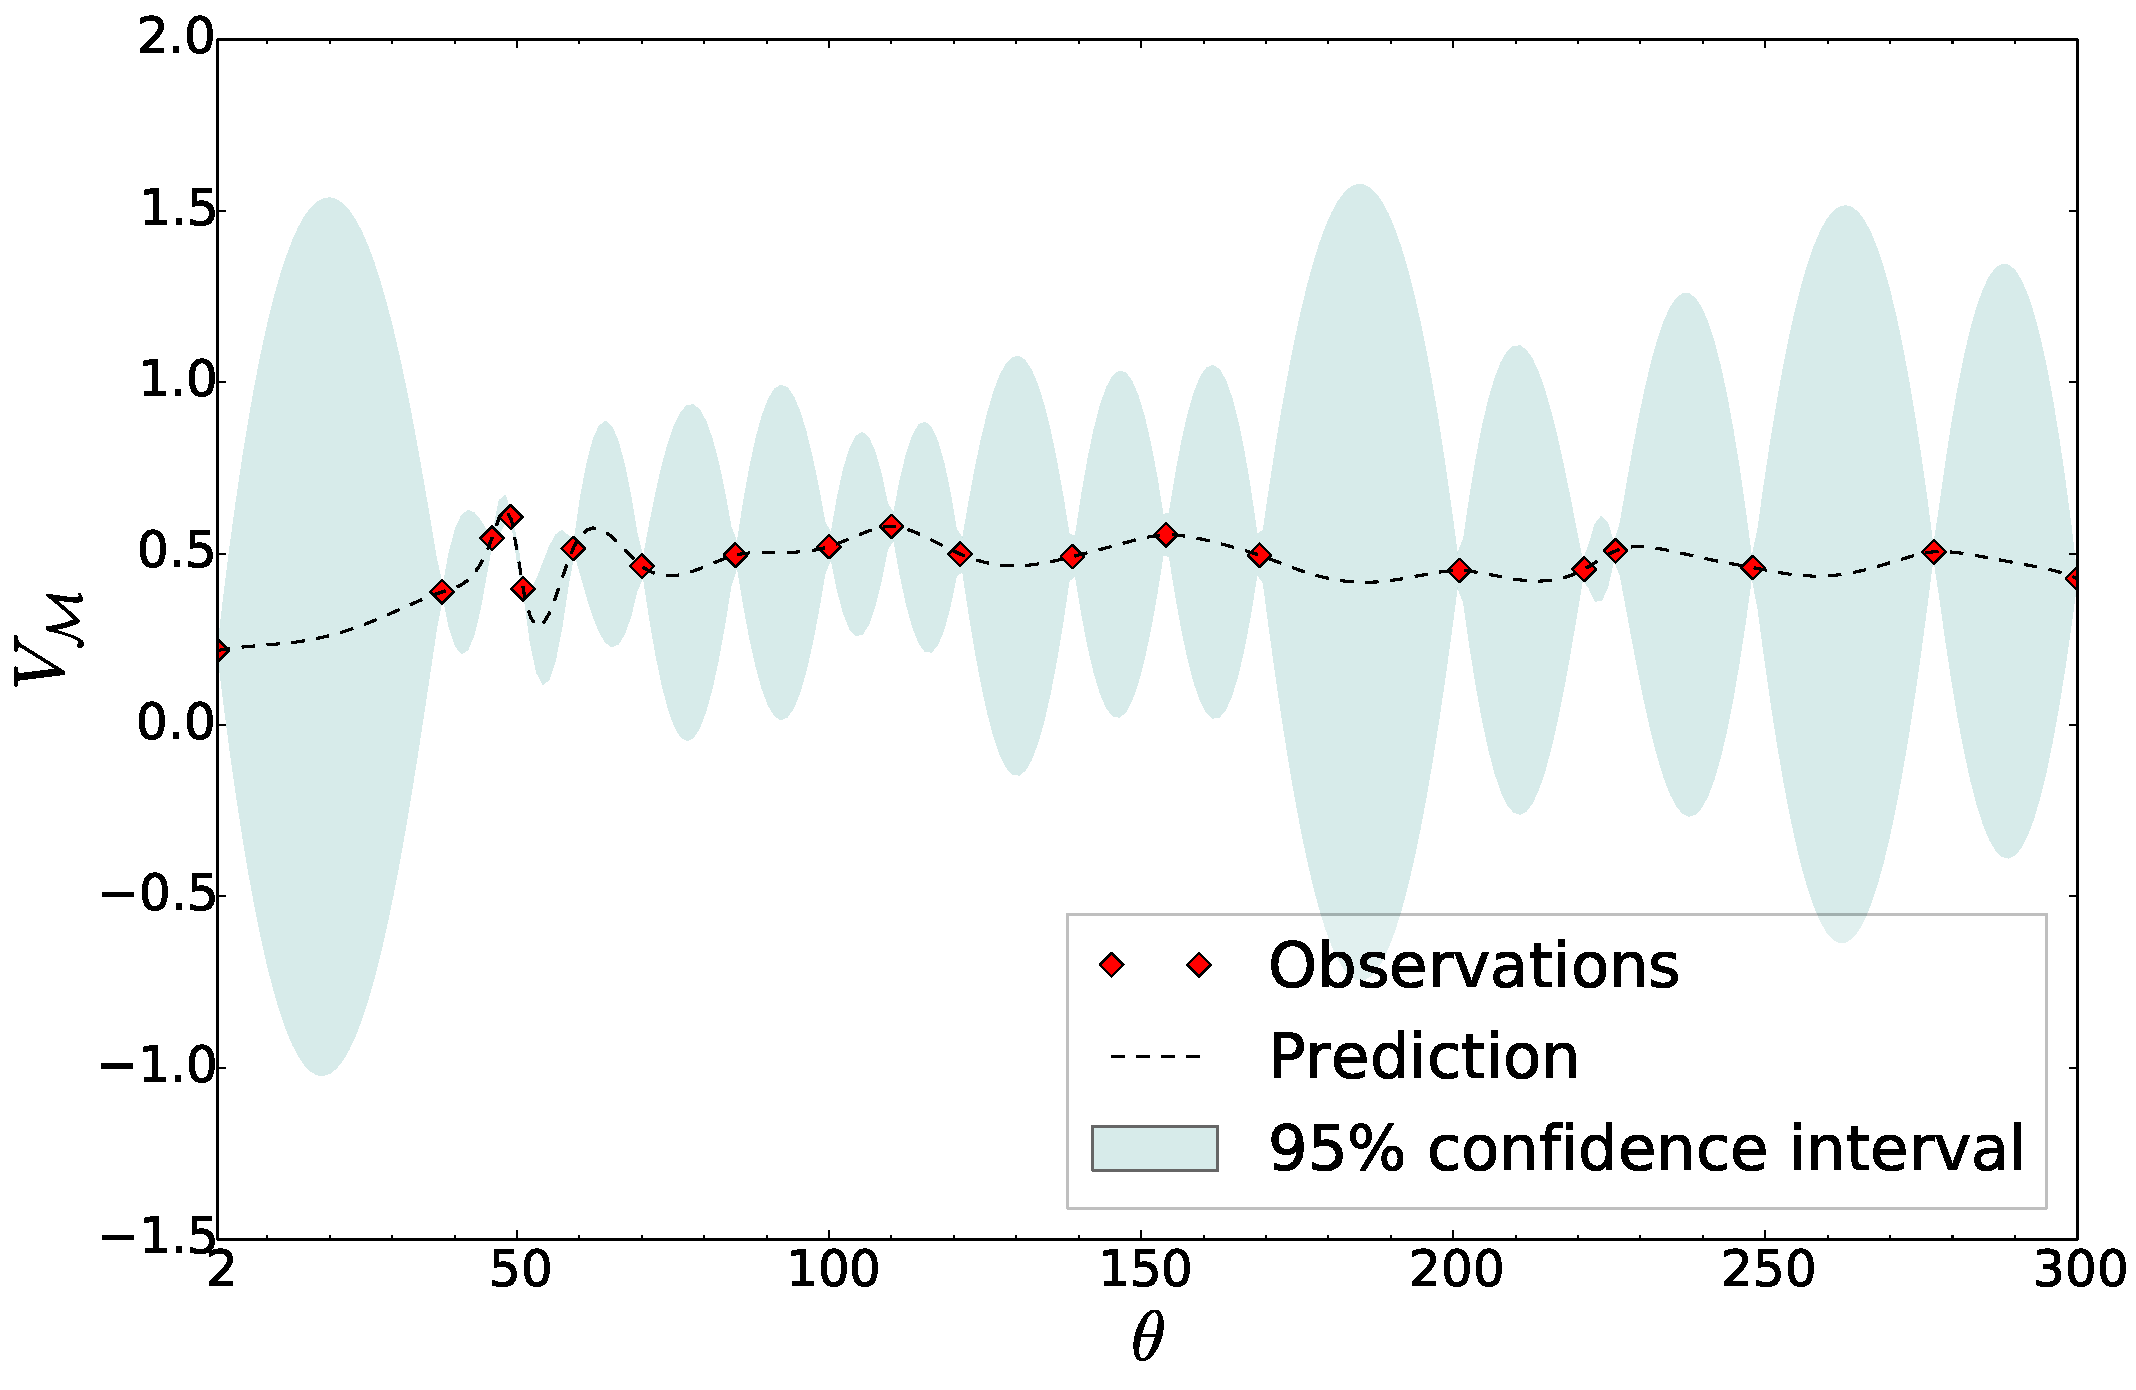
\includegraphics[width=0.9\textwidth]{plots/tum_base/plot_b_00__alg_kmeans_pct_50_acq_ei}
		\caption{Plot showing posterior after 20 iterations of the optimization routine for the \texttt{tum\_kitchen} environment, $\beta = 0.0$, $k$-Means, $50\%$ of the dataset used, \acrshort{acr:mei} acquisition function used (Experiment 3).}
		\label{fig:exp3}
	\end{figure}
	\clearpage
}

First of all, let us consider the results obtained for the small \texttt{tum\_kitchen} environment.
Overall, in \Crefrange{fig:exp1}{fig:exp9} one can see that the optimum $\theta_\mathsf{max}$ found lies mostly, with a few explainable exceptions, in the same area of the parameter space.
In \Crefrange{fig:exp1}{fig:exp3} respectively 100\%, 75\% and 50\% of the dataset has been used in the corresponding experiments, and one can see here that with 50\% almost no distinction can be made in assessed performance.
At the other hand, \autoref{fig:exp2} shows that with 75\% of the data the distinction becomes much more clear.
What might explain this, is that this particular section of the dataset adds data based on which \acrshortpl{acr:mdp} with large state spaces overfit their corresponding transition function.

	% ID = 4
	\begin{figure}
		\centering
		\includegraphics[width=0.9\textwidth]{plots/tum_base/plot_b_00__alg_kmeans_pct_100_acq_ucb}
		\caption{Plot showing posterior after 20 iterations of the optimization routine for the \texttt{tum\_kitchen} environment, $\beta = 0.0$, $k$-Means, $100\%$ of the dataset used, \acrshort{acr:gp-ucb} acquisition function used (Experiment 4).}
		\label{fig:exp4}
	\end{figure}
	% ID = 5
	\begin{figure}
		\centering
		\includegraphics[width=0.9\textwidth]{plots/tum_base/plot_b_00__alg_kmeans_pct_100_acq_eips}
		\caption{Plot showing posterior after 20 iterations of the optimization routine for the \texttt{tum\_kitchen} environment, $\beta = 0.0$, $k$-Means, $100\%$ of the dataset used, \acrshort{acr:mei-ps} acquisition function used (Experiment 5).}
		\label{fig:exp5}
	\end{figure}

Next, let us compare the results depicted in \autoref{fig:exp1}, \autoref{fig:exp4} and \autoref{fig:exp5} where different acquisition functions are used in the \acrshort{acr:bo} framework (i.e., \acrshort{acr:mei}, \acrshort{acr:gp-ucb} and \acrshort{acr:mei-ps} respectively).
For this environment, we see the results are quite similar, and also in the logs made from the experiments it was seen that the maximum observation was done in the (exact) same number of steps (in the third step).
The most clear difference is seen in the `behavior' of the acquisition functions from the logs, which show that \acrshort{acr:mei-ps} first samples the points for which model learning and planning is less expensive.

Then, in \autoref{fig:exp6} and \autoref{fig:exp7} we see the plots for the experiments in which \acrshortpl{acr:gmm} are used for learning state spaces instead.
In particular we notice the low model-values for a large number of components of the \acrshort{acr:gmm}, which makes us suspect that this particular algorithm is less suitable for learning state spaces for our domain.

\afterpage{
	% ID = 6
	\begin{figure}[t!]
		\centering
		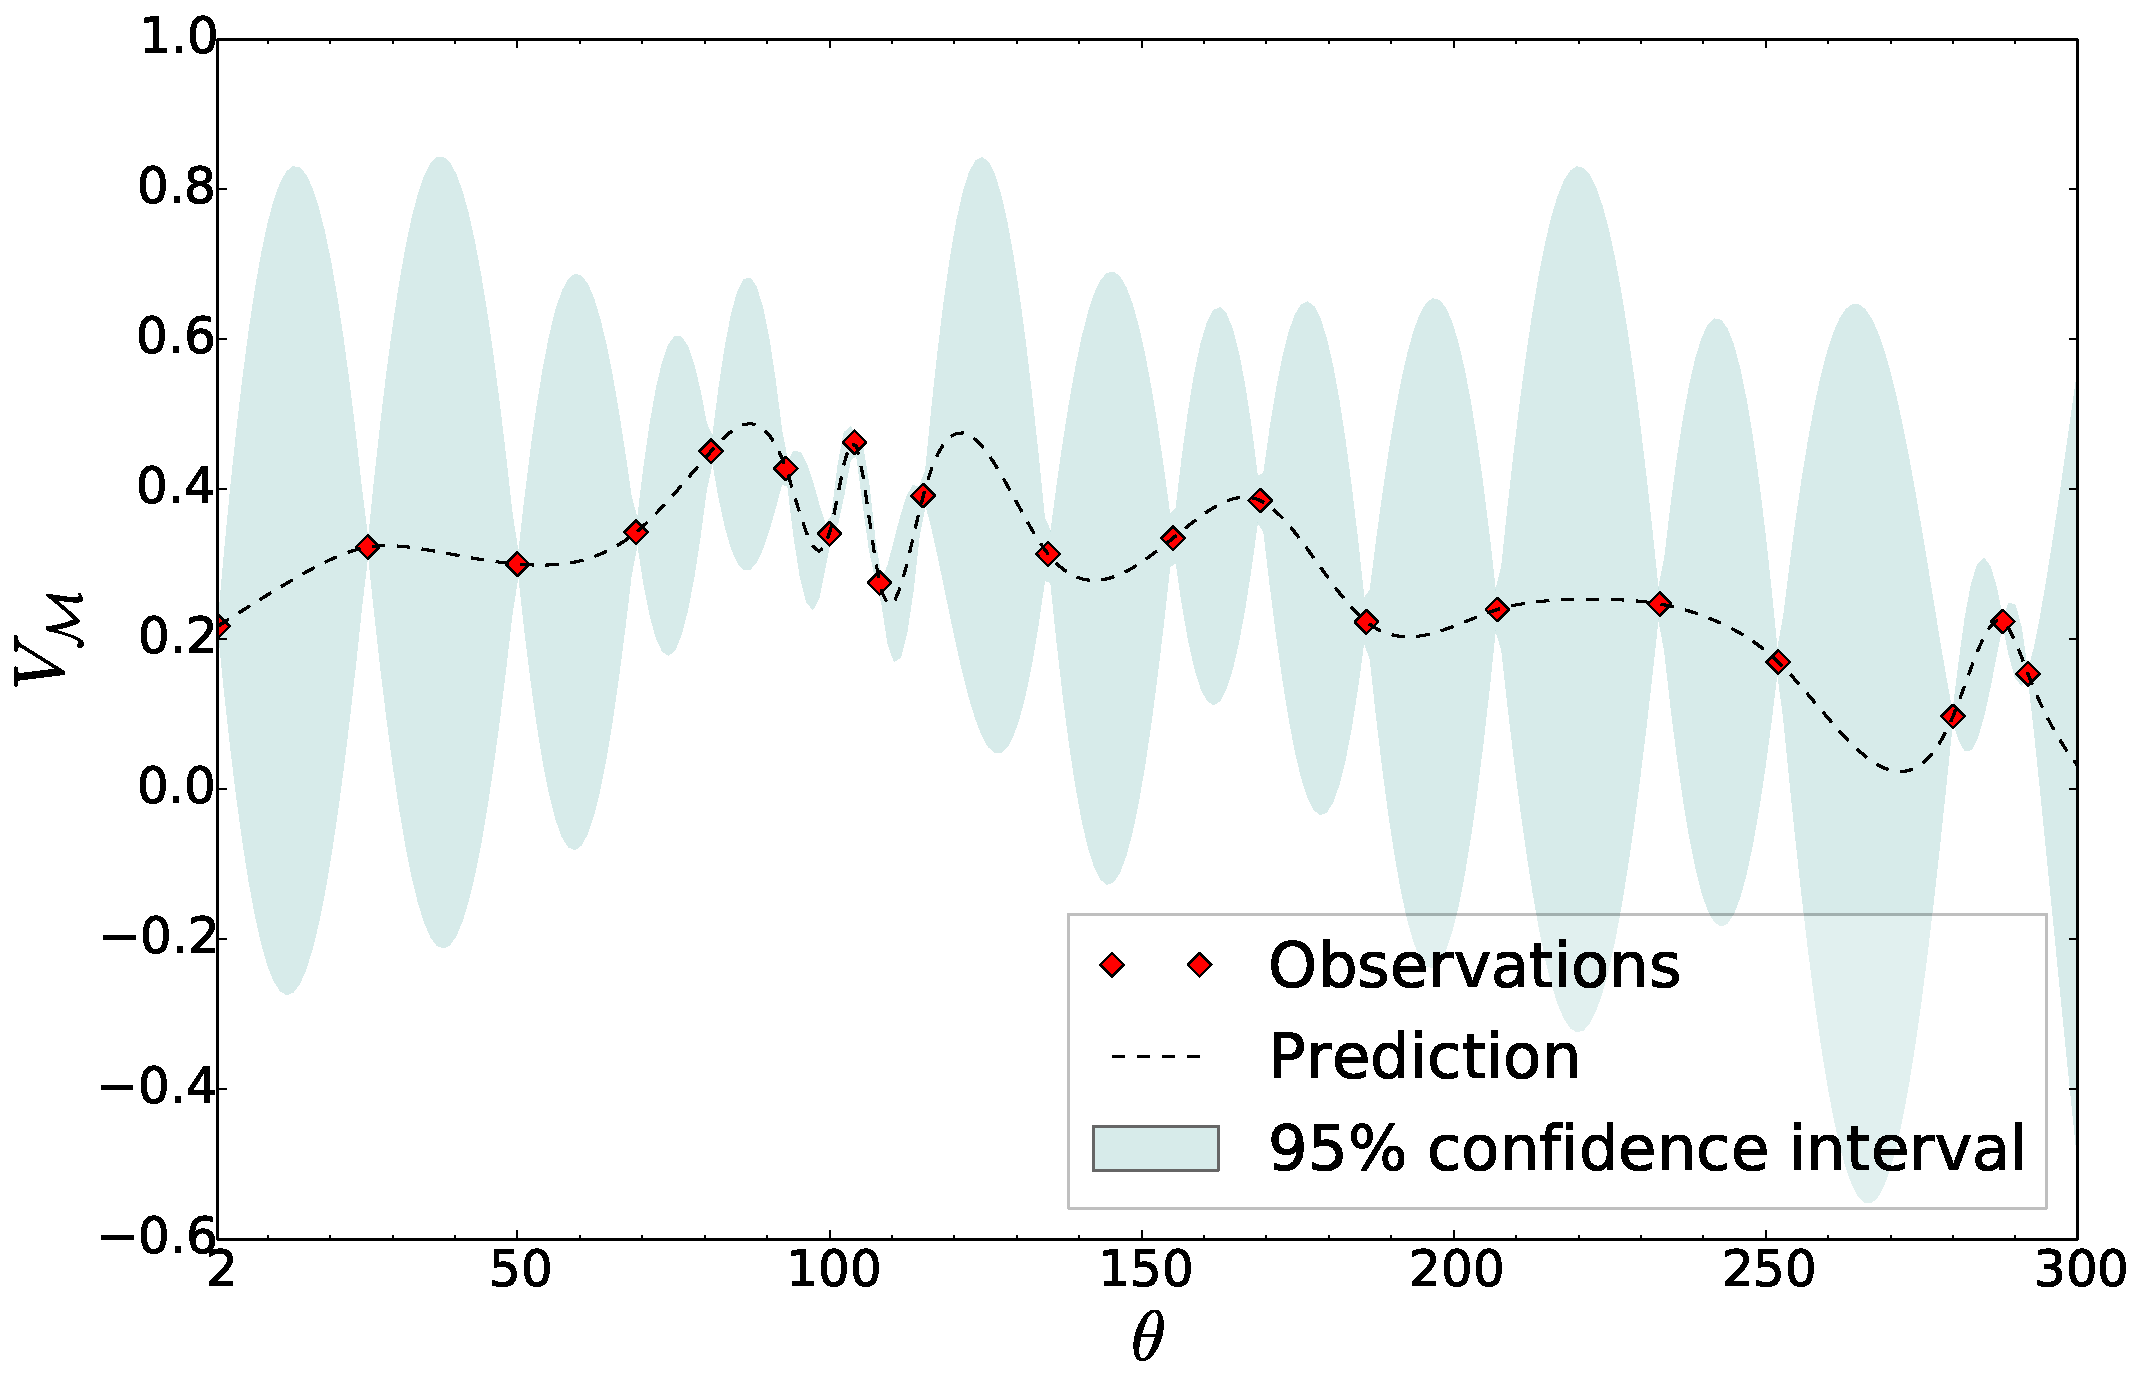
\includegraphics[width=1.0\textwidth]{plots/tum_base/plot_b_00__alg_gmm_pct_100_acq_ei}
		\caption{Plot showing posterior after 20 iterations of the optimization routine for the \texttt{tum\_kitchen} environment, $\beta = 0.0$, \acrshort{acr:gmm}, $100\%$ of the dataset used, \acrshort{acr:mei} acquisition function used (Experiment 6).}
		\label{fig:exp6}
	\end{figure}
	% ID = 7
	\begin{figure}[t!]
		\centering
		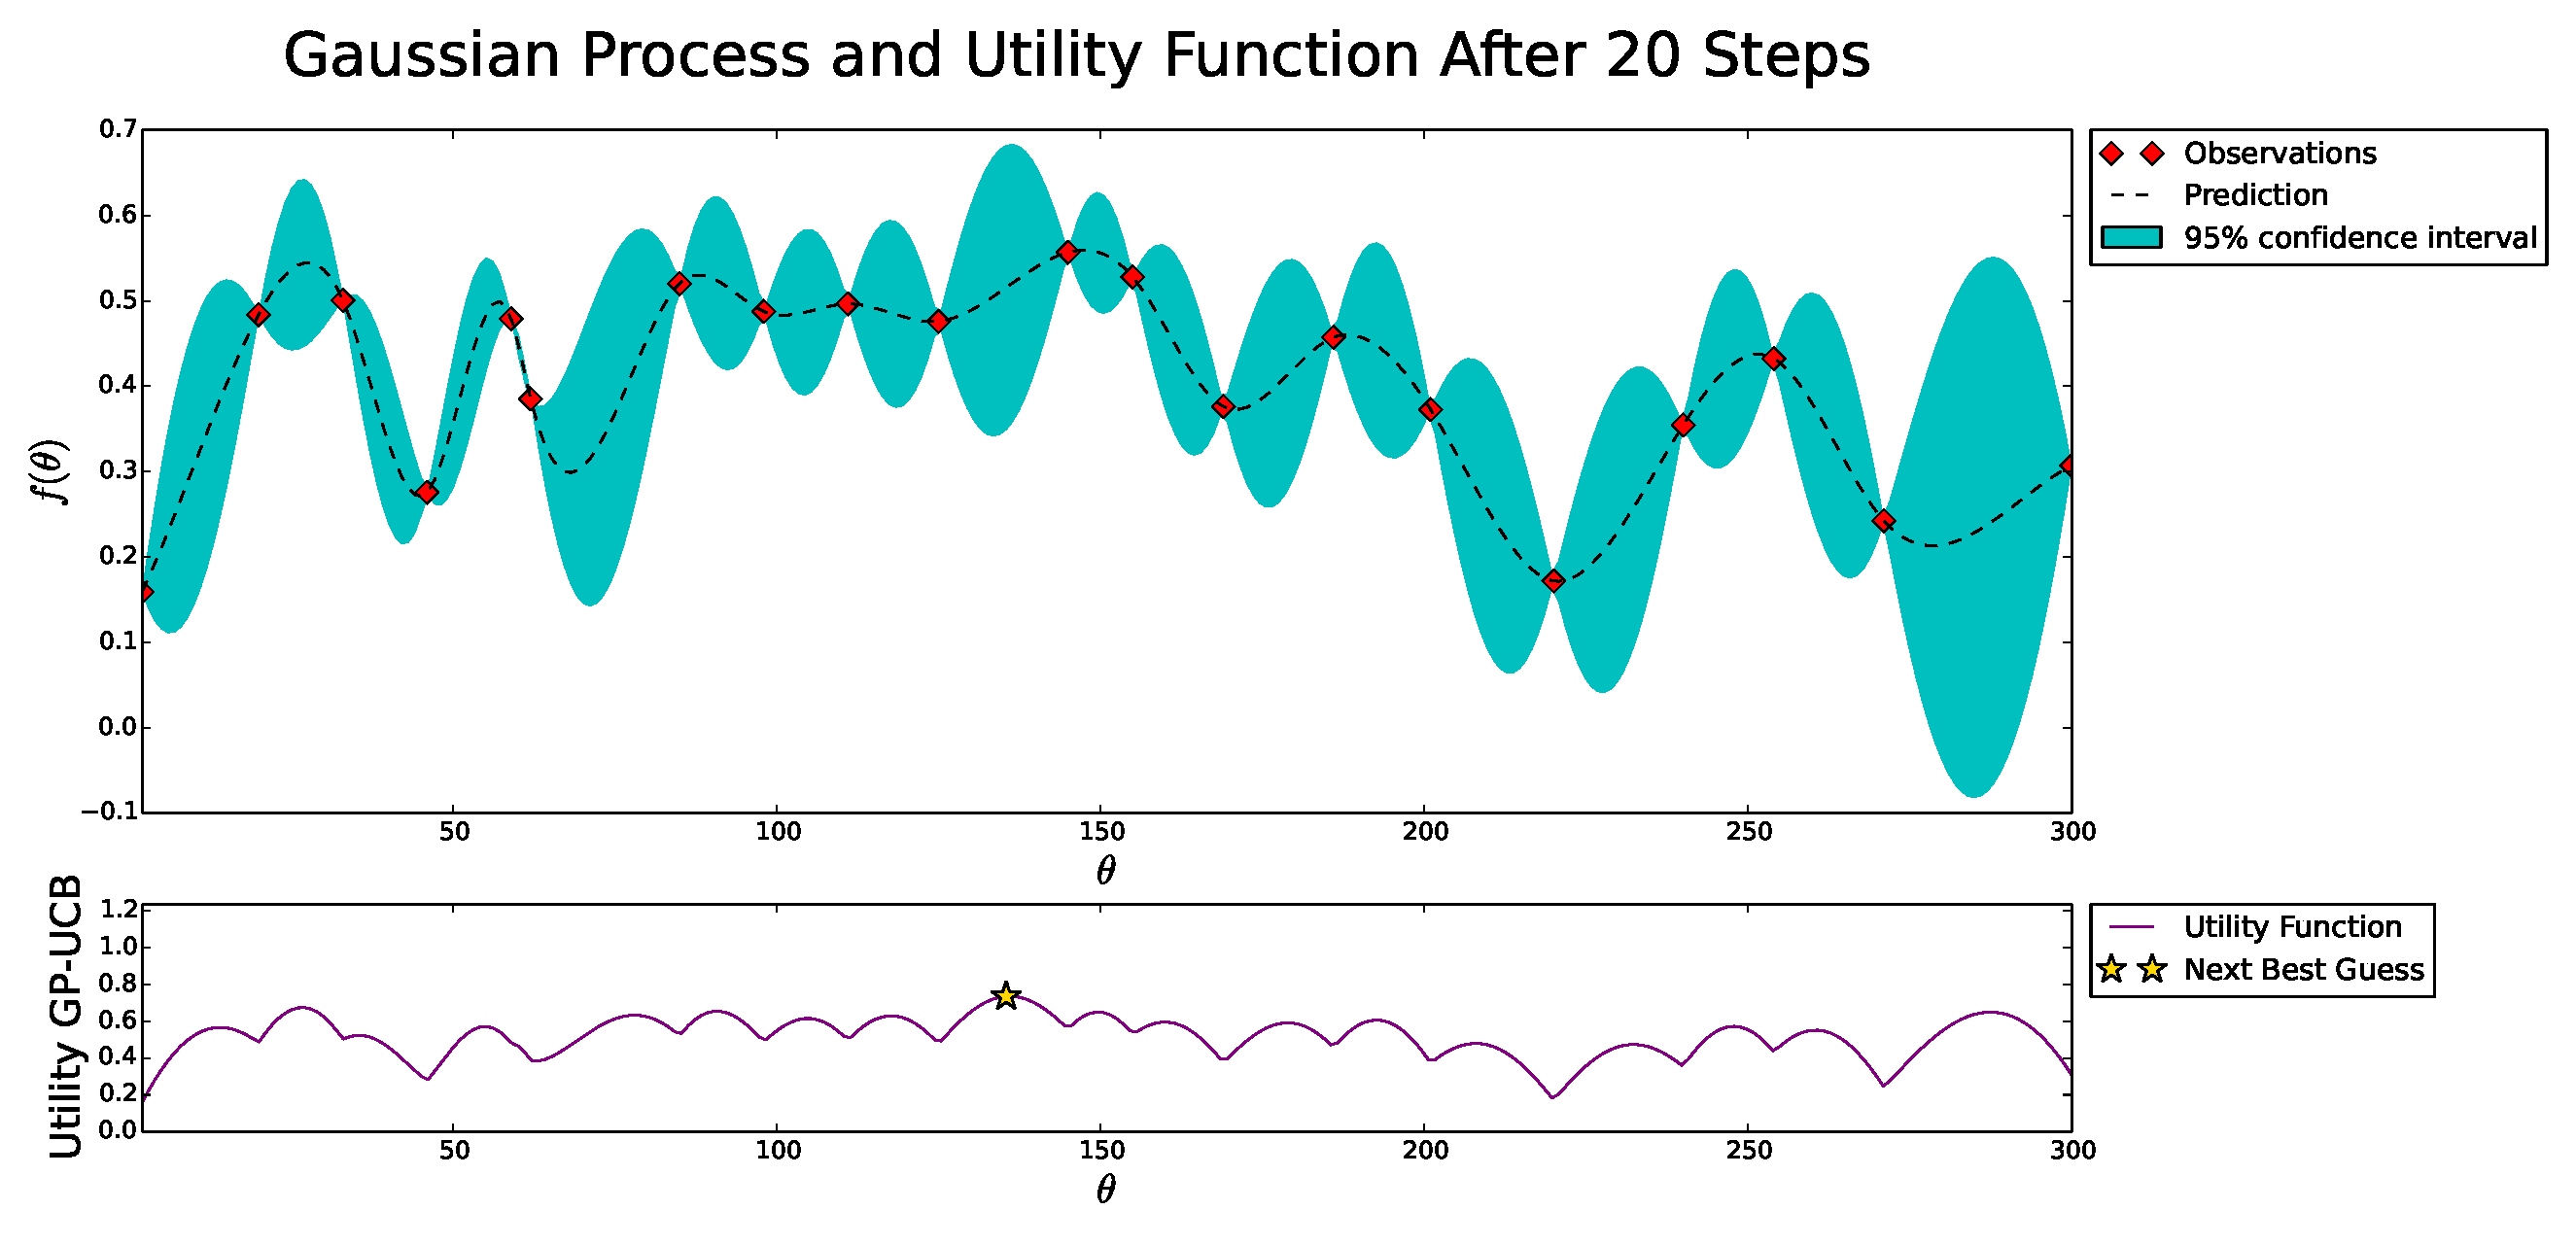
\includegraphics[width=1.0\textwidth]{plots/tum_base/plot_b_00__alg_gmm_pct_100_acq_ucb}
		\caption{Plot showing posterior after 20 iterations of the optimization routine for the \texttt{tum\_kitchen} environment, $\beta = 0.0$, $k$-Means, $100\%$ of the dataset used, \acrshort{acr:gp-ucb} acquisition function used (Experiment 7).}
		\label{fig:exp7}
	\end{figure}
	\clearpage
}

\newpage
	
Finally, we look at the influence of the weight factor $\beta$ for the small environment considering the plots of \autoref{fig:exp1}, \autoref{fig:exp8} and \autoref{fig:exp9}.
In this particular situation, one might benefit from weighing $V_\mathit{DTP}$ in the model-value, as it could make a clearer distinction between values for different settings for $\theta$.
However, setting $\theta$ might also lead to a bias, which is that although $V_\mathit{DTP}$ may have high value, computed policies may not work well in the simulations or the real world.

	% ID = 8
	\begin{figure}[t!]
		\centering
		\includegraphics[width=1.0\textwidth]{plots/tum_base/plot_b_025__alg_kmeans_pct_100_acq_ei}
		\caption{Plot showing posterior after 20 iterations of the optimization routine for the \texttt{tum\_kitchen} environment, $\beta = 0.25$, $k$-Means, $100\%$ of the dataset used, \acrshort{acr:mei} acquisition function used (Experiment 8).}
		\label{fig:exp8}
	\end{figure}
	% ID = 9
	\begin{figure}[t!]
		\centering
		\includegraphics[width=1.0\textwidth]{plots/tum_base/plot_b_05__alg_kmeans_pct_100_acq_ei}
		\caption{Plot showing posterior after 20 iterations of the optimization routine for the \texttt{tum\_kitchen} environment, $\beta = 0.5$, $k$-Means, $100\%$ of the dataset used, \acrshort{acr:mei} acquisition function used(Experiment 9).}
		\label{fig:exp9}
	\end{figure}

Then, let us next consider the results for the large \texttt{uol\_bl} environment. In \Crefrange{fig:exp10}{fig:exp12} plots are shown for the experiments in which different acquisitions were used in the \acrshort{acr:bo}.
One can observe that the optima found after 20 steps are quite different, which might indicate that more steps are necessary to move towards a global optimum for each of these experiments.

\afterpage{
	% ID = 10
	\begin{figure}[t!]
		\centering
		\includegraphics[width=0.9\textwidth]{plots/uol_base/plot_b_00__alg_kmeans_pct_100_acq_ei}
		\caption{Plot showing posterior after 20 iterations of the optimization routine for the \texttt{uol\_bl} environment, $\beta = 0.0$, $k$-Means, $100\%$ of the dataset used, \acrshort{acr:mei} acquisition function used (Experiment 10).}
		\label{fig:exp10}
	\end{figure}
	% ID = 11
	\begin{figure}[t!]
		\centering
		\includegraphics[width=0.9\textwidth]{plots/uol_base/plot_b_00__alg_kmeans_pct_100_acq_ucb}
		\caption{Plot showing posterior after 20 iterations of the optimization routine for the \texttt{uol\_bl} environment, $\beta = 0.0$, $k$-Means, $100\%$ of the dataset used, \acrshort{acr:gp-ucb} acquisition function used (Experiment 11).}
		\label{fig:exp11}
	\end{figure}
	% ID = 12
	\begin{figure}[t!]
		\centering
		\includegraphics[width=0.9\textwidth]{plots/uol_base/plot_b_00__alg_kmeans_pct_100_acq_eips}
		\caption{Plot showing posterior after 20 iterations of the optimization routine for the \texttt{uol\_bl} environment, $\beta = 0.0$, $k$-Means, $100\%$ of the dataset used, \acrshort{acr:mei-ps} acquisition function used (Experiment 12).}
		\label{fig:exp12}
	\end{figure}
	\clearpage
}

\newpage

\subsection{Multiphase Framework}
\label{sec:multiphase-framework-results}

In \Crefrange{fig:exp13}{fig:exp18} one can see that optima are found within the same area of the parameter space as seen in the results for the base framework. However the logs do not show the pre-processing influencing the area of interest in the second phase.

\vspace{12pt}
\noindent\fbox{\textbf{TODO:} Fix problems most likely in implementation for the multi-phase framework for more usable results.}

\afterpage{
	% ID = 13
	\begin{figure}[t!]
		\centering
		\includegraphics[width=0.9\textwidth]{plots/tum_multi/plot_b_00__alg_kmeans_pct_100_acq_ei}
		\caption{Plot showing posterior after 20 iterations of the optimization routine for the \texttt{tum\_kitchen} environment, $\beta = 0.0$, $k$-Means, $100\%$ of the dataset used, \acrshort{acr:mei} acquisition function used (Experiment 13).}
		\label{fig:exp13}
	\end{figure}
	% ID = 14
	\begin{figure}[t!]
		\centering
		\includegraphics[width=0.9\textwidth]{plots/tum_multi/plot_b_025__alg_kmeans_pct_100_acq_ei}
		\caption{Plot showing posterior after 20 iterations of the optimization routine for the \texttt{tum\_kitchen} environment, $\beta = 0.25$, $k$-Means, $100\%$ of the dataset used, \acrshort{acr:mei} acquisition function used (Experiment 14).}
		\label{fig:exp14}
	\end{figure}
	% ID = 15
	\begin{figure}[t!]
		\centering
		\includegraphics[width=0.9\textwidth]{plots/tum_multi/plot_b_05__alg_kmeans_pct_100_acq_ei}
		\caption{Plot showing posterior after 20 iterations of the optimization routine for the \texttt{tum\_kitchen} environment, $\beta = 0.5$, $k$-Means, $100\%$ of the dataset used, \acrshort{acr:mei} acquisition function used (Experiment 15).}
		\label{fig:exp15}
	\end{figure}
	\clearpage
}

\afterpage{
	% ID = 16
	\begin{figure}[t!]
		\centering
		\includegraphics[width=0.9\textwidth]{plots/uol_multi/plot_b_00__alg_kmeans_pct_100_acq_ei}
		\caption{Plot showing posterior after 20 iterations of the optimization routine for the \texttt{uol\_bl} environment, $\beta = 0.0$, $k$-Means, $100\%$ of the dataset used, \acrshort{acr:mei} acquisition function used (Experiment 16).}
		\label{fig:exp16}
	\end{figure}
	% ID = 17
	\begin{figure}[t!]
		\centering
		\includegraphics[width=0.9\textwidth]{plots/uol_multi/plot_b_025__alg_kmeans_pct_100_acq_ei}
		\caption{Plot showing posterior after 20 iterations of the optimization routine for the \texttt{uol\_bl} environment, $\beta = 0.25$, $k$-Means, $100\%$ of the dataset used, \acrshort{acr:mei} acquisition function used (Experiment 17).}
		\label{fig:exp17}
	\end{figure}
	% ID = 18
	\begin{figure}[t!]
		\centering
		\includegraphics[width=0.9\textwidth]{plots/uol_multi/plot_b_05__alg_kmeans_pct_100_acq_ei}
		\caption{Plot showing posterior after 20 iterations of the optimization routine for the \texttt{uol\_bl} environment, $\beta = 0.5$, $k$-Means, $100\%$ of the dataset used, \acrshort{acr:mei} acquisition function used (Experiment 18).}
		\label{fig:exp18}
	\end{figure}
	\clearpage
}

% Small state-spaces: discrepancy between goal state and true goal is discounted
% Large state-spaces overshooting + overfitting on limited training data